\chapter{Utveckling av webbsida}
\label{sec: webb}

Inom produktutveckling är det viktigt att arbeta iterativt för att gradvis förbättra kvalitén på produkten. Under utvecklingen av webbsidan har därför en strukturerad iterationsprocess varit nödvändig. I detta kapitel ges först en kort introduktion till produkt- och webbutveckling och vår övergripande iterationsprocess. Därefter presenteras resultatet. På grund av arbetets utformning har vi valt att utgå ifrån iterationsprocessen i hur vi strukturerar och presenterar resultatet. Avslutningsvis diskuterar vi arbetsprocessen och vidare arbete. 


\section{Förhållningspunkter, bakgrund och metodik}
Arbetets utformning skapar utmaningen att med en användarcentrerad utveckling skapa en fullt fungerande, flexibel och skalbar webbsida på kortast möjliga tid. Webbsidan måste vara fullt fungerande av två skäl. För det första måste den användas i en riktig situation för att samla in data över studenternas studiemönster. För det andra behöver webbsidan vara fullt fungerande för att möjliggöra testning av funktionalitet och för att kontrollera att den uppfyller användarens behov och krav. Flexibilitet är en viktig förhållningspunkt för att kunna experimentera med ny funktionalitet. Därtill bör webbsidan vara skalbar, vilket innebär möjligheten att öka antalet kurser och användare på sidan, utan att skapa administrativa problem. Till sist är tidskravet viktigt eftersom arbetet begränsas av de tidsgränser som sätts av kurserna som webbsidan används i.

% Arbetets utformning skapar utmaningen att på snabbast möjliga tid, med en användarcentrerad utveckling, skapa en fullt fungerande och skalbar webbsida. Webbsidan måste vara fullt fungerande av två skäl. För det första måste den användas i en riktig situation för att få verklig data på studenternas studiemönster. För det andra behöver webbsidan vara fullt fungerande för att möjliggöra testning av ny funktionalitet och kontollera att den uppfyller användarens behov och krav. Webbsidan bör också vara skalbar, vilket innebär möjlighet att öka antalet kurser och användare på sidan, utan att skapa administrativa problem. Tidskravet är viktigt eftersom projektet förhåller sig till de tidsgränser som de faktiska kurserna sätter, såsom kursstart och tentavecka. 

Genom att utgå från användarfeedback kan utvecklingen av webbsidan bättre anpassas till användarens behov och krav. För ett sådant arbetssätt krävs en strukturerad metodik. Nedan beskrivs den övergripande processen för arbetssättet, samt några specifika metoder. Därefter beskrivs ett fåtal centrala begrepp inom webbutveckling, samt de ramverk som har använts för att ta fram webbsidan. 


\subsection{Produktutveckling: metoder och begrepp}
I ett produktutvecklingsarbete behöver det initialt samlas in information om användaren och användningssituationen. I den initiala fasen används metoder som intervjuer, enkäter och observationer. Sedan krävs en analys av den insamlade informationen för att få en djupare förståelse för användaren och situationen. Under analysen används statistiska metoder vid stora mängder kvantitativ data. Om informationen består av verbal data, från exempelvis öppna enkätfrågor eller intervjusvar, finns utarbetade metoder för att bearbeta informationen. \emph{KJ-analys} är ett exempel på en sådan metod \cite{kj}. Därefter sker en fas av idégenerering. Med utgångspunkt från den insamlade och bearbetade informationen tas lösningar och koncept fram på de problem och behov som har identifierats. Slutligen väljs ett av koncepten. Valet kan göras med hjälp av utarbetade metoder, men också utifrån utvecklarnas eget omdöme om vad som anses rimligt givet tid, resurser och kontext. 

Intervju är en frågebaserad metod för att få fram information ifrån användaren. För att få information av hög kvalité är det viktigt att typen av intervju, frågorna, och urvalet av intervjuobjekt tas i beaktande. Det finns exempelvis \emph{strukturerade intervjuer}, \emph{semistrukturerade intervjuer}, och \emph{ostrukturerade intervjuer}. I en strukturerad intervju går utfrågaren igenom en på förhand utarbetad intervjumall. En semistrukturerad intervju utgår från en intervjumall, men utrymme ges för utvikningar på ämnen som kommer upp. Den semistrukturerade intervjun kännetecknas av fler följdfrågor för att få intervjuobjektet att utveckla sina svar. Ostrukturerade intervjuer utgår inte från en förbestämd intervjumall, utan är snarare ett öppet samtal kring ett förutbestämt ämne. 

KJ-analys är en metod för att strukturera stora mängder verbal information. Metoden kan användas för att gruppera användarbehov och krav i hierarkier, som sedan kan representeras i ett träddiagram. Resultatet är en grafisk bild av helheten, som samtidigt illustrerar samband mellan olika delar. Tillvägagångssättet är att successivt bygga upp en struktur genom att kategorisera de svar som mottagits. För varje enskilt svar, från exempelvis en öppen enkätfråga, ställs frågan om det svaret hör ihop med något av de tidigare svaren. Om ja, placeras svaret tillsammans i den identifierade kategorin. Om nej, får svaret utgöra en ny kategori. Vid repetition för samtliga svar kan de skapade kategorierna namnsättas och viktiga förhållanden kan sedan dras emellan dem. 

En minimalt funktionell produkt (eng. \emph{Minimum Viable Product}) eller \emph{MVP} är en produkt med precis tillräckligt många funktioner för att tillfredsställa tidiga användare och förse utvecklarna med information för vidare produktutveckling. En MVP är ett mer tidseffektivt och billigare sätt att testa idéer och koncept än att bygga en produkt med mer komplett funktionalitet \cite{ries}. 

\subsection{Webbutveckling: begrepp och ramverk}
Webbutveckling kan enkelt beskrivas som utvecklingen av applikationer, vars primära syfte är att visas och användas i en webbläsare. En webbapplikation kan förenklat delas upp i två delar: framsida (eng. \emph{front end}) och serversida (eng. \emph{server side} eller ibland \emph{back end}). Framsidan är vad användaren ser och kan interagera med. Serversidan är logik på servar som användarna inte ser eller direkt kan interagera med, såsom databashantering, autentisering och svarsvalidering.

Med tiden har metoder för webbutveckling förbättrats och utvecklats. Ett exempel är framsideramverket \emph{React} \cite{react}, och används exempelvis för att förenkla, snabba upp, och möjliggöra skalbar utveckling av webbsidor. Förenklandet och skalbarheten uppnås bland annat genom en komponentbaserad modell som gör det lättare att återanvända och analysera delar av applikationen. Ökningen i hastighet sker genom Reacts sätt att uppdatera den aktuella vyn. React uppdaterar endast de komponenter som har förändrats vilket sparar tid då inte alla delar behöver målas ut på nytt.

\emph{GraphQL} är ett frågespråk (eng. \emph{query language}), som används vid kommunikation till serversido-applikationer \cite{graphql}. Dessa applikationer används ofta för att hantera koppling mot databaser. Ett annat vanligt sätt att implementera kopplingen är genom att använda metodiken REST. REST är ett engelskt akronym för \emph{Representational State Transfer}, som beskriver en metodik för att hantera transaktioner mellan digitala maskiner \cite{rest}. En nackdel med applikationer som använder sig av REST är att de ofta bygger på en förutbestämd struktur, vilket skapar beroenden och långsamma iterationsprocesser. Enkelt förklarat behöver utvecklare ofta i förväg definiera hur en applikation är tänkt att användas, och behöver därför lägga till slutpunkter (eng. \emph{endpoints}) för nya användarfall. GraphQL löser detta problem som uppstår med REST, genom att via en datagraf (eng. \emph{data graph}) möjliggöra en lösare koppling mellan användarfall och implementation. Utvecklingen beror då inte på enskilda slutpunkter, utan tillåter istället en mer flexibel informationshantering.

\subsection{Iterationsprocess}

\begin{wrapfigure}{r}{0.43\textwidth}
  \begin{center}
    \resizebox {0.4\textwidth} {!} {
        \definecolor{klight_green_400}{RGB}{156, 204, 101}

\tikzset{%
  project part/.style={
    rectangle,
    draw,
    fill=klight_green_400,
    thick,
    minimum width=3.2cm,
    minimum height=1.2cm
  },
  main line/.style={
    draw,
    line width=1mm,
    opacity=1,
    minimum size=1cm
  },
}

\begin{tikzpicture}[x=1.5cm, y=1.5cm, ->,>=stealth',auto, thick, line width=0.5mm, every node/.style={scale=1.3}]
% Base project nodes
\node [project part/.try] (collect) at (2,2) {$\textbf{Information}$};
\node [project part/.try] (concept) at (0,0) {$\textbf{Koncept}$};
\node [project part/.try] (use) at (4,0) {$\textbf{Användning}$};
\node [project part/.try] (implement) at (2,-2) {$\textbf{Implementation}$};


% Connect them 
\path[main line/.style={font=\sffamily\small}]
    (collect) edge[bend right] node[align=center, xshift=-1mm] [left] {\large KJ-analys, \\ \large idégenerering} (concept)
    (concept) edge[bend right] node [left] {\large Figma} (implement)
    (implement) edge[bend right] node[align=center, xshift=1mm] [right] {\large React, \\ \large GraphQL} (use)
    (use) edge[bend right] node[align=center, xshift=1mm] [right] {\large Intervjuer, \\ \large statistik} (collect);
\end{tikzpicture}
    }
    \caption{Iterationsprocess för produkt-  och webbutveckling. Figuren visar de huvudsakliga stegen och kopplingarna däremellan.}
    \label{fig:iteration_process}
  \end{center}
\end{wrapfigure}

För att optimera utvecklingen krävdes en tydlig iterationsprocess. Vår valda iterationsprocess presenteras i figur \ref{fig:iteration_process} och utgår från fyra huvudmoment. Processen inleds med en informationsinsamling. Utifrån insamlad information analyseras behov och krav, som sedan ligger till grund för att ta fram en mängd olika koncept. I konceptmomentet väljs ett av koncepten för att gå vidare med och en grafisk prototyp av konceptet skapas i visualiseringsprogrammet \emph{Figma} \cite{figma}. Därefter används Figma-prototypen som en utgångspunkt för att implementera det föreslagna konceptet i kod. Implementationen till kod utförs med hjälp av React och GraphQL. Iterationsprocessen avslutas med att det implementerade konceptet tillgängliggörs för användare. Användningen möjliggör sedan ytterligare informationsinsamling, varpå nästa cykel kan påbörjas. 


\section{Iterationscykler}

I arbetet genomförde vi två cykler av iterationsprocessen. I den första iterationscykeln tog vi fram en grundläggande MVP för webbsidan. I den andra iterationcykeln utökades föregående funktionalitet till det vi kallar för MVP A. Nedan presenteras de två iterationcyklerna separat.

\subsection{Iterationscykel 1: grundläggande MVP}
I iterationscykel 1 bestod informationsinsamlingen av en undersökning av programmen MapleTA och OpenTA. Vi analyserade även inlärningsprogrammen \emph{Duolingo} \cite{duolingo} och \emph{Khan Academy} \cite{khanacademy} för att få en uppfattning om rådande gränssnittsdesign och funktionalitet.

Specifikt utförde vi intervjuer med föreläsare, samt utvärderingar med studenter kring programmen OpenTA och MapleTA. Till exempel genomförde vi ett test i en kurs på kandidatnivå där studenterna kunde använda OpenTA frivilligt genom att kursens rekommenderade uppgifter var inlagda i programmet. Detta test utvärderades med en enkät i slutet av kursen. Vi utförde också en KJ-analys på de öppna enkätsvaren. Enkäten fick 62 svar och sammanställningen av resultatet går att se i Appendix \ref{app:opentasurvey}. Från resultatet noterade vi exempelvis att studenterna uppskattade funktionalitet såsom automaträttning och direkt återkoppling (eng. \emph{immediate feedback}), men även att de uppskattade den struktur och översikt programmet gav deras studier. Något som studenterna däremot upplevde att de saknade var lösningsförlag och tips när de fastnar i lösningsgången. Ett exempel på resultatet från KJ-analyserna av de öppna frågorna går att se i figur \ref{fig:raket1}. Här syns exempelvis att studenterna tyckte översikten underlättade, samt att de uppskattade automaträttningen.

\begin{figure}[hbtp]
    \centering
    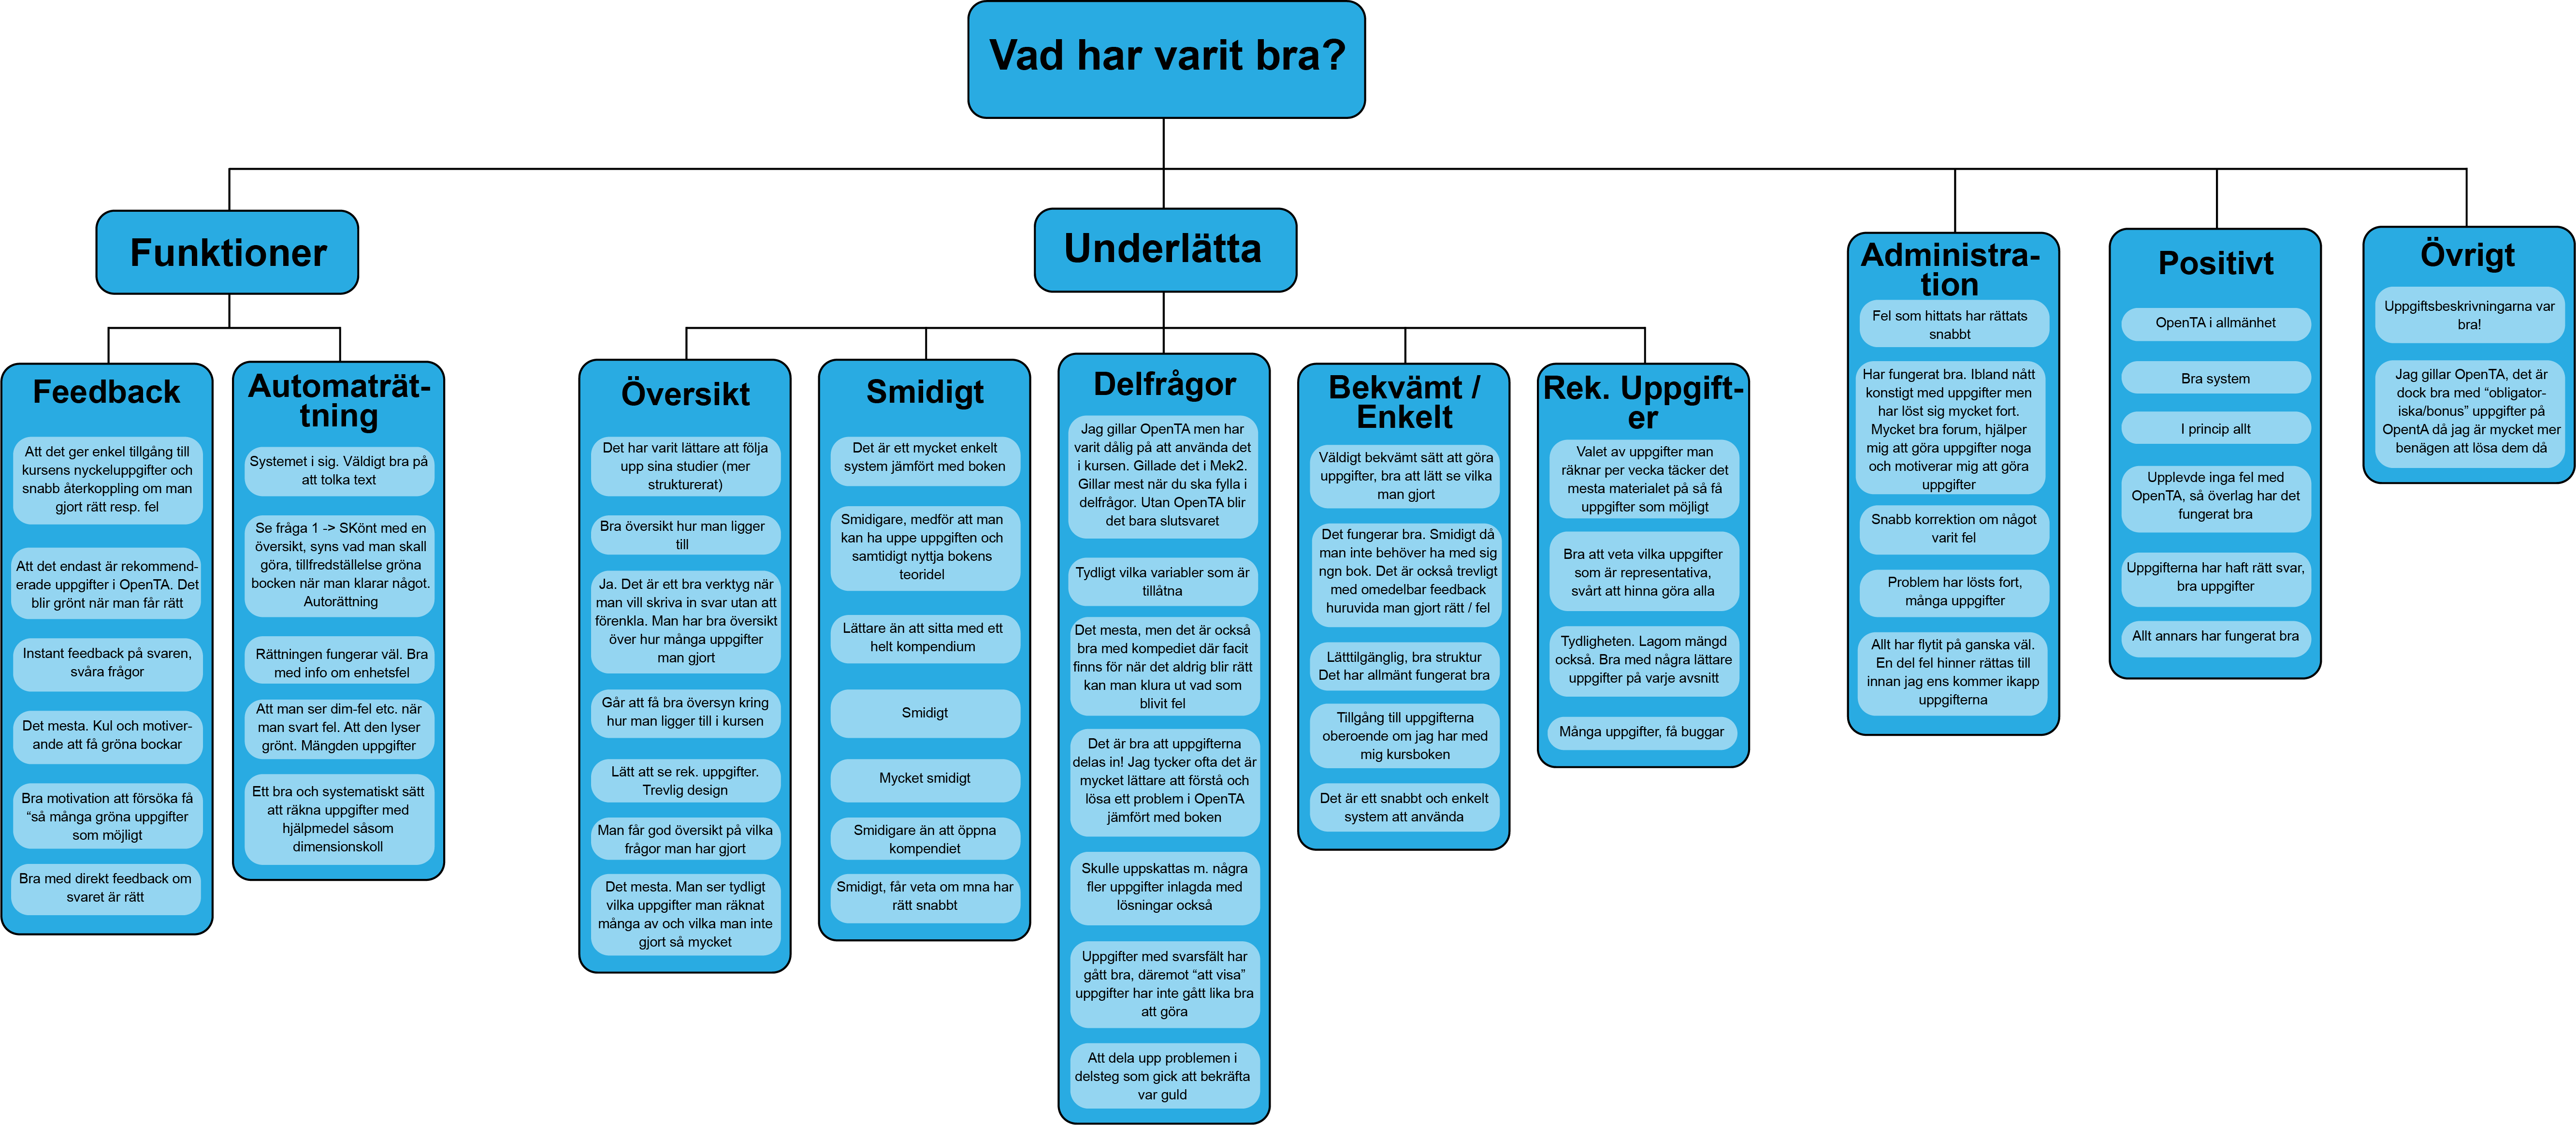
\includegraphics[width=1\textwidth]{images/resultpictures/opentakj.png}
    \caption{Resultatet av KJ-analysen från svaren på frågan ''Vad har varit bra?''. Specifikt visar rubrikerna de övergripande sambanden i enkätsvaren, medan de enkilda svaren representerar andelen svar per rubrik. För en version med fullständigt läsbara svar, se Appendix \ref{app:kjOpenTA}.}
    \label{fig:raket1}
\end{figure}




I analysen av programmen Doulingo och Khan Academy fokuserade vi specifikt på användargränssnittet och funktionalitet. En klar trend vi såg var att vara tydlig med återkoppling till användaren visuellt. Exempelvis i form av gröna bockar vid korrekt svar eller progressionsfält (eng. \emph{progression bars}), som visar även de minsta framsteg. Ytterligare insikter vi fick var att hålla gränssnittet avskalat och inte dölja några element. 

Därefter gick arbetet vidare till konceptfasen. Utifrån informationen från intervjuer, enkäter, KJ-analys, samt analysen av inlärningsprogrammen skapade vi en grafisk prototyp av webbsidans gränssnitt i Figma, vilket utgjorde en grund för utvecklandet av den grundläggande MVP:n. I resterande del av det här avsnittet presenterar vi designen och funktionaliteten i den grundläggande MVP:n. För att följa iterationsprocessen inleder vi med att jämföra frågevyn från den grafiska prototypen med implementationen av samma vy på webbsidan. Därefter beskriver vi den övergripande strukturen på hela webbsidan och presenterar designvalen mer ingående. Dessutom beskriver vi hur designvalen har implementerats.

I figur \ref{fig:raket2} presenteras en tvådelad bild med frågevyn som designades i Figma ovanför implementationen av vyn på webbsidan. Notera att de olika elementen i den grafiska prototypen överensstämmer i stor utsträckning med motsvarande element i implementationen. Överst i frågevyn ges vilken uppgift användaren befinner sig på samt ett progressionsfält som förmedlar hur stor andel av uppgifterna som är lösta. Därunder lyfts uppgifttexten och eventuell bild fram på en vit bakgrund för att framhålla fokus. I övrigt är andra element avskalade för att undvika plottrighet och distraktion enligt insikterna från informationsinsamlingen. 

\begin{figure}[hbtp]
    \centering
    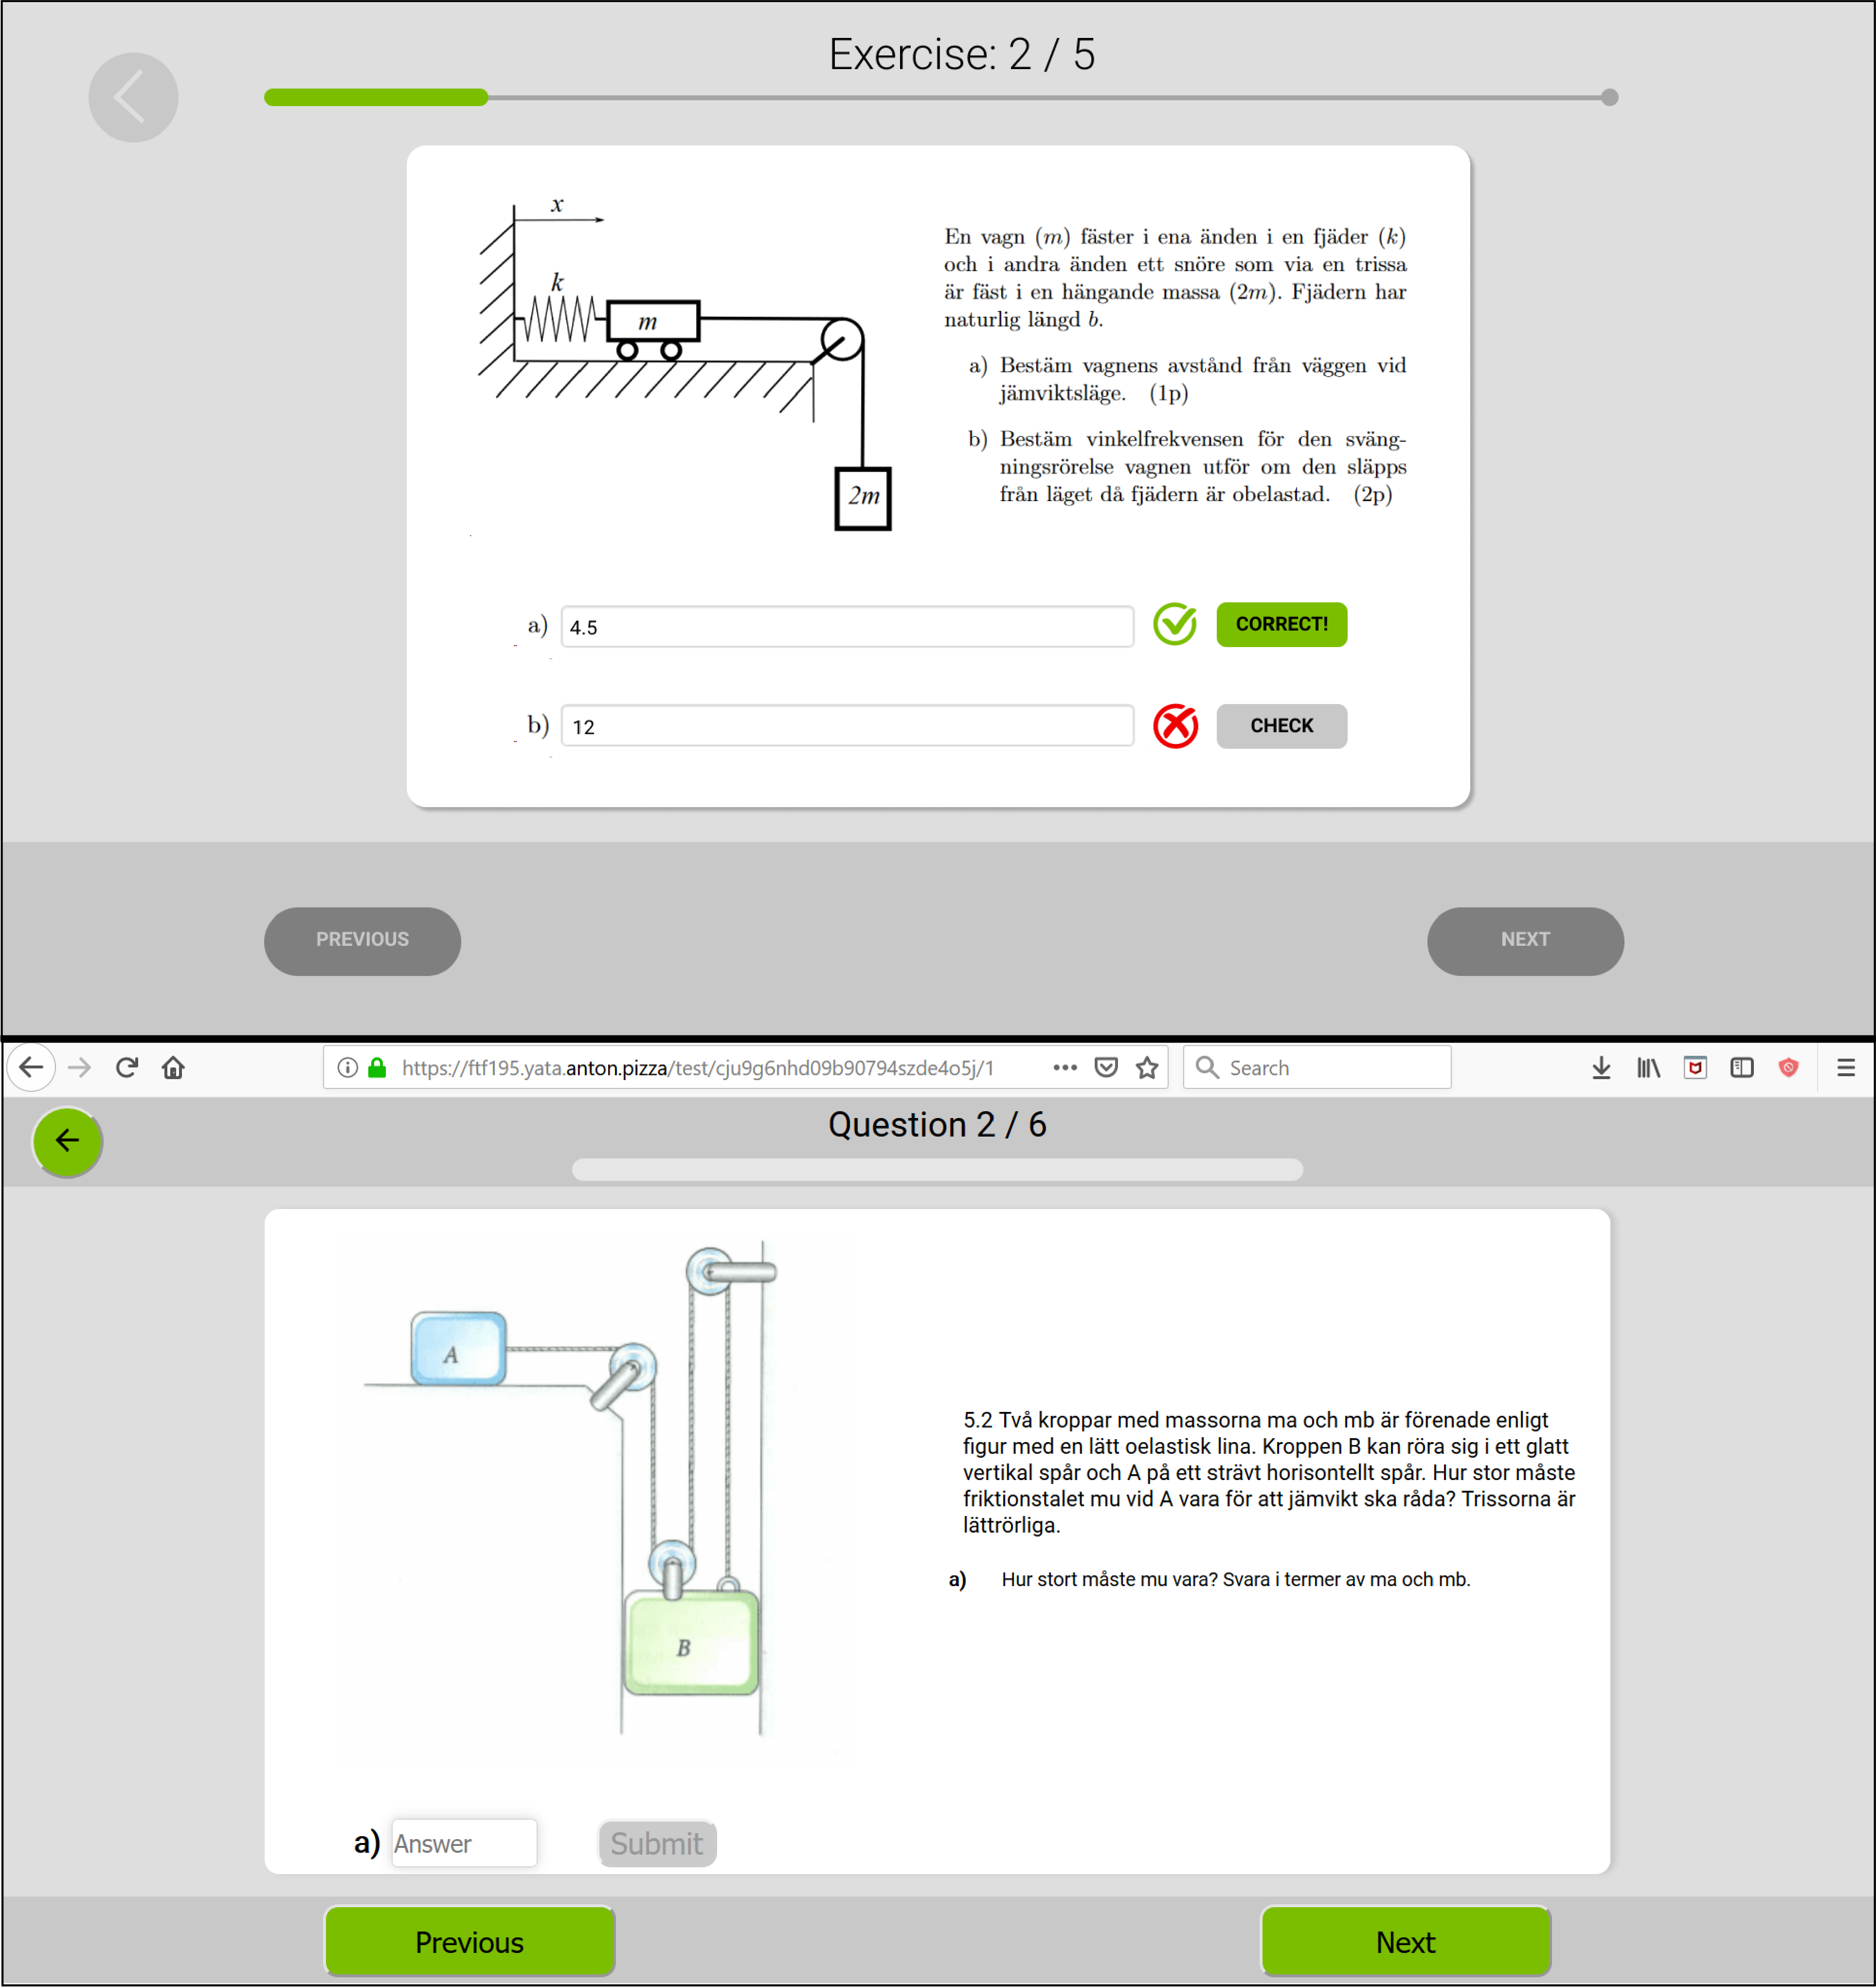
\includegraphics[width=0.95\textwidth]{images/resultpictures/figmaweb2.png}
    \caption{En grafisk design skapad i Figma av frågevyn (övre bild) med motsvarande implementation som visad i en webbläsare (undre bild).}
    \label{fig:raket2}
\end{figure}

Implementationsfasen av den grundläggande MVP:n resulterade i applikationen \emph{YetAnotherTA}, förkortat YATA. En demoversion av webbsidan är tillgänglig på \url{https://demo.yata.anton.pizza}, där användarnamnet ''demo'' används för inloggning. För att interaktivt följa med i beskrivningen av webbsidans övergripande struktur rekommenderar vi läsaren att använda demoversionen. 

Webbsidan är uppdelad i fyra olika vyer: login-skärm (1), kapitelvy (2), översiktsvy (3) samt frågevy (4) vilka visas i figur \ref{fig:raket4}. Eftersom studenterna i informationsinsamlingen visade sig uppskatta översikt och struktur är detta något som har prioriterats i designen. Efter att ha loggat in via login-skärmen ska användaren i kapitelvyn snabbt kunna få en överskådlig bild över hur den ligger till i kursen. Detta genom att användaren ser de olika kapitlen samt hur stor del av uppgifterna i ett kapitel som är lösta, vilket representeras av en procentsats samt ett progressionsfält. För varje kapitel finns en översiktsvy över de olika uppgifterna i kapitlet. Där syns hur många uppgifter kapitlet innehåller samt vilka som är lösta respektive olösta. Överst i översiktsvyn finns också ett progressionsfält som visar andelen lösta uppgifter i kapitlet. I frågevyn kan sedan användaren navigera mellan de olika uppgifterna i kapitlet med hjälp av knapparna \emph{Next} och \emph{Previous}. Användaren kan återgå till översiktsvyn från frågevyn genom tillbakapilen i övre vänstra hörnet. På samma sätt kan användaren komma från översiktsvyn till kapitelvyn. 

\begin{figure}[hbtp]
    \centering
    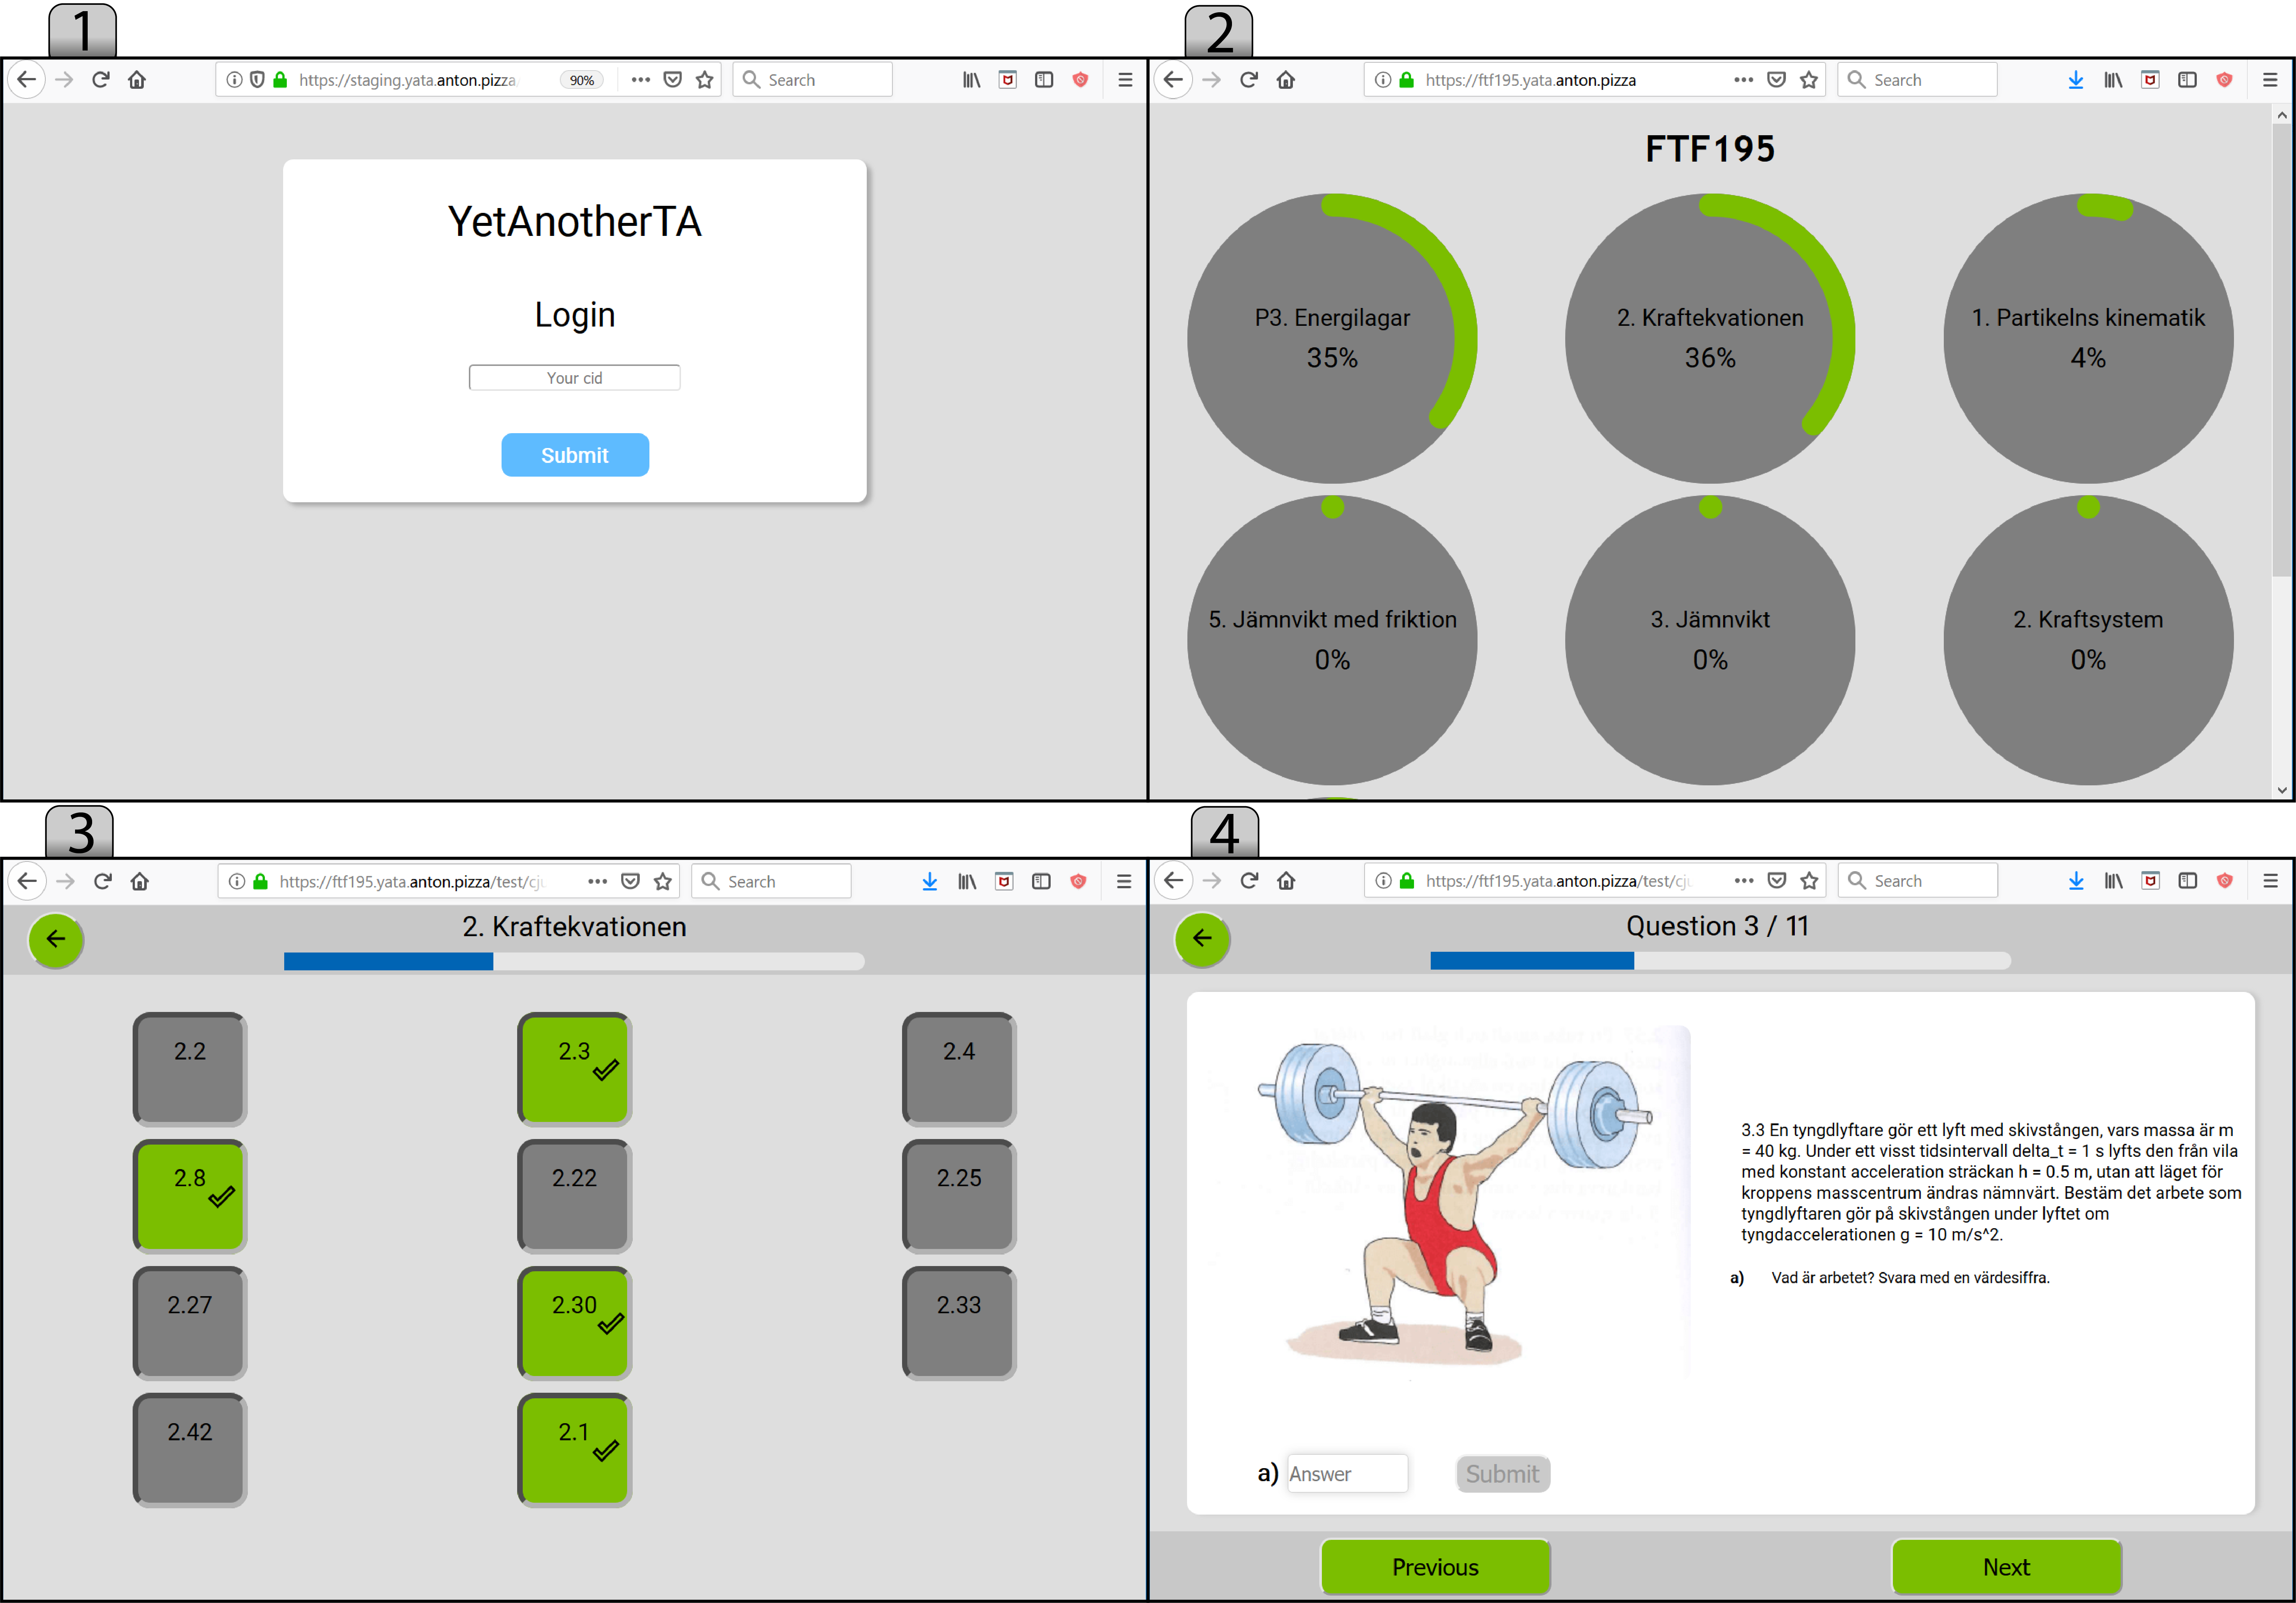
\includegraphics[width=1.0\textwidth]{images/resultpictures/4pics1website.png}
    \caption{De fyra olika vyerna i den grundläggande MVP:n. Vyerna är numrerade enligt: 1. login-skärmen, 2. kapitelvyn, 3. överisktsvyn och 4. frågevyn. }
    \label{fig:raket4}
\end{figure}

%%%%%%% TEKNISKT 

%%% "Den är uppbyggd på ett väldigt generellt sätt... kurskord... courseview... hittar själv... bidrar till skalbarhet då vi inte behöver ändra något för nya kurser
Implementationen av webbsidan i kod bygger på en generell struktur. Varje kurs tilldelas ett unikt ID som används för att hämta uppgiftssamlingar från databasen genom GraphQL, som sedan målas ut på vyerna med hjälp av React. På grund av den generella strukturen kan en ny kurs snabbt registreras på en ny webbadress. Det enda som behövs är ett namn på kursen samt tillhörande samling av räkneuppgifter. Därmed är det enkelt att lägga till nya kurser vilket bidrar till skalbarheten.

När användaren skriver in sitt användarnamn i login-skärmen skickas en nätverksförfrågan till GraphQL. Om användaren inte finns registrerad på kursen återfås ett felmeddelande, men annars omdirigeras användaren till kapitelvyn för tillgängliga uppgiftssamlingar. I kapitelvyn kan användaren välja bland de samlingar av uppgifter som presenteras, exempelvis som kapitel ur en lärobok, veckans rekommenderade uppgifter, eller en gammal tentamen. När användaren klickar på vald samling uppgifter kommer samlingens ID att hämtas med GraphQL för att dirigera användaren till översiktsvyn. Översiktsvyn visar samtliga frågor i uppgiftsamlingen och användaren kan även se vilka frågor som är besvarade. Komponenten som översiktsvyn är baserad på är uppbyggd på samma sätt som föregående kapitelvy. Uppgifter hämtas med GraphQL och målas ut som fyrkanter på vyn, vilka är gröna ifall de har besvarats. Alla uppgifter sparas i cache-minnet. Det medför att användaren kommer nå frågevyn för en specifik uppgift direkt utan att behöva vänta på en ny hämtning, vilket gör navigeringen snabbare.

Komponenten som hanterar frågevyn är dynamiskt programmerad, vilket innebär att den anpassar innehållet till skärmens storlek. I nedre delen av skärmen finns knappar för navigering mellan frågorna. Som tidigare nämnts är alla frågor sparade i cache-minnet, vilket gör att navigationen mellan uppgifter upplevs momentan. Efter att användaren fyllt i och skickat sitt svar anropas GraphQL som sparar svaret, tidpunkten för svaret och ifall det var rätt eller fel i databasen. Responsen återkopplas sedan till användaren i form av en grön bock eller ett rött kryss beroende på om svaret var korrekt eller felaktigt. Informationen som sparas i databasen kan sedan användas av den artificiella intelligensen som presenteras i kapitel \ref{sec:Deep}.

Den grundlägganden MVP:n testades sedan i slutet av läsperiod 3 i två matematiktunga kurser på kandidatnivå genom att lägga in gamla tentamina på webbsidan och frivilligt låta kursernas studenter använda den. Insamlade resultat utvärderas och analyseras som start i iterationscykel 2.

\subsection{Iterationscykel 2: MVP A}
Efter iterationscykel 1 utvärderade vi den grundläggande MVP:n med hjälp av ostrukturerade intervjuer. Totalt intervjuades sju studenter och intervjuerna spelades in och transkriberades. Synpunkter från intervjuerna återkopplades till utvecklingen. Två exempel på synpunkter vi fick var att inmatningsfälten borde förstoras och att svar bör stå kvar i inmatningsfältet då användaren lämnar uppgiften och kommer tillbaka senare. Den fulla listan med förbättringspunkter återges i Appendix \ref{app:itt}. 

Parallellt med utvecklingen av grundfunktionaliteten gjorde vi en användarstudie av plattformen \emph{Piazza}, som är ett forum där studenter kan ställa frågor och få svar från andra studenter eller föreläsare. Användarstudien utfördes för att samla in ytterligare information kring problematiken att många studenter kör fast i sina lösningsgångar. Ett urval gjordes av nio studenter från Teknisk fysik på Chalmers tekniska högskola från årskurserna 1-5. Detta för att Piazza använts i flera kurser på Teknisk fysik, samt för att få insikt i om åsikterna skiljer sig emellan årskurserna. Semistrukturerade intervjuer hölls med deltagarna, se Appendix \ref{app:surveypiazza} för intervjumall. Intervjuerna transkriberades varefter nyckelcitat extraherades och en KJ-analys utfördes på dessa. En sammanställning av KJ-analysen går att finna i Appendix \ref{app:KJ-analys}. Slutsatsen från användarstudien var att forumet inte användes i någon större utsträckning av studenterna. Vi identifierade flera anledningar till detta. Exempelvis upplevdes svarstiden lång. Ögonblicklighet är därav ett av kraven vi upptäckte i användarstudien.

Ögonblickligheten är även en orsak till en hierarki vi identifierade i hur studenter söker efter hjälp när de kört fast. Hierarkin presenteras i figur \ref{fig:raket5}. Trenden är att studenterna börjar söka på Google efter lösningar på problem då de fastnar. Om hjälp inte hittas där är ett vanligt nästa steg att studenterna frågar nära vänner via en chatt, exempelvis en gruppchatt på Facebook. Hjälper heller inte det, är nästa steg att studenterna frågar andra studiekamrater nära till hands. Till sist använder studenterna Piazza om de fortfarande behöver hjälp. Vår tolkning av detta är att studenterna värdesätter svarstiden högre än kvalitén på svaren. Att fråga på Piazza hade förmodligen genererat ett svar av hög kvalité, dock upplevs svarstiden ofta lång. Ett citat från en av intervjuerna är ''det känns bättre att googla i fem minuter än att vänta i fem minuter'', vilket visar på ett tydligt behov av att få hjälpen direkt.

\begin{figure}[hbtp]
    \centering
    \hspace{-20px}
    \resizebox {1\textwidth} {!} {
        \definecolor{klight_green_400}{RGB}{156, 204, 101}



\begin{tikzpicture}[x=1.5cm, y=1.5cm, ->,>=stealth',auto, thick, line width=0.5mm]
\tikzset{%
  project part/.style={
    rectangle,
    draw,
    fill=klight_green_400,
    thick,
    minimum width=3.2cm,
    minimum height=1.2cm
  },
  main line/.style={
    draw,
    line width=0.25mm,
    opacity=1,
    minimum size=1cm
  },
}
% Base project nodes
\node [project part/.try] (control) at (0,0) {$\textbf{Google}$};
\node [project part/.try] (predict) at (3,0) {$\textbf{Gruppchatt}$};
\node [project part/.try] (form) at (6,0) {$\textbf{Kursare}$};
\node [project part/.try] (interview) at (9,0) {$\textbf{Piazza}$};


% Connect them 
\path[main line/.style={font=\sffamily\small}]
    (control) edge[right] node [left] {} (predict)
    (predict) edge[right] node [left] {} (form)
    (form) edge[right] node [left] {} (interview);
\end{tikzpicture}

    }
    \caption{En representation av hierarkin i vilken många studenter söker efter hjälp. För en bild av den fullständiga KJ-analysen där denna hierarki identifierades, se Appendix \ref{app:KJ-analys}. }
    \label{fig:raket5}
\end{figure}

En bidragande orsak till hierarkin är sociala faktorer. Vi observerade att studenterna överlag drar sig för att ställa frågor i större öppna forum. Det finns en viss social rädsla för att fråga om hjälp i mer offentliga sammanhang, även om det är i en digital miljö som ett forum. Studenterna upplever att en mindre gruppchatt med sina nära vänner är en tryggare miljö än Piazza. Jämförelsevis är inte Google en social miljö på samma sätt som ett forum eller en gruppchatt, vilket tar bort den sociala rädslan. Att Google används som det första steget i hierarkin tolkar vi som att det finns ett behov av att minska de sociala faktorerna för att studenter ska söka hjälp. Därav drar vi slutsatsen att anonymitet utgör ytterligare ett krav på koncept som försöker lösa problemet om att studenter kör fast i sina lösningsgångar.

%Studenterna känner sig tryggare att fråga om hjälp i en mindre gruppchatt med sina nära vänner. Istället söker många först hjälp via Google. Möjligtvis för att Google är mest lättillgängligt, men kanske också för att det inte är en social miljö på samma sätt som ett forum eller en gruppchatt. 

Utifrån den insamlade informationen samt de identifierade behoven och kraven föreslogs ett antal koncept, se Appendix \ref{app:koncept}. Det koncept vi slutligen bestämde oss för, kallad MVP A, är en typ av tipsfunktion. Implementationen av konceptet visas i figur \ref{fig:raket6} och kan även testas på demoversionen av webbsidan. Tipsfunktionen valdes på grund av flera av de tidigare presenterade observationerna. Till exempel efterfrågades tips av studenterna i utvärderingen av OpenTA. Tipsfunktionen är även anonym och utgör inte en social miljö samtidigt som funktionen erbjuder ögonblicklig hjälp. Funktionen kräver dock att tips finns skrivna och vår tanke är att tipsen ska genereras av studenterna själva. Detta genom att de som löst en uppgift får möjlighet att skriva in ett tips på den uppgiften som sedan kan användas av någon som har kört fast på samma uppgift. En uppgift ska kunna ha flera tips vilket gör att en typ av rangordning behöver finnas. Vår tanke är att användarna ska kunna ge ett tips en ''tumme upp'' eller en ''tumme ner''. På så vis kan det högst rankade tipset visas först för studenten vid begäran av ett tips. Dessutom möjliggör tipsfunktionen ett ytterligare sätt att samla in data över studenternas studier till utvecklingen av den artificiella intelligensen. Till exempel information om hur många som begär och skriver tips.

\begin{figure}[hbtp]
    \centering
    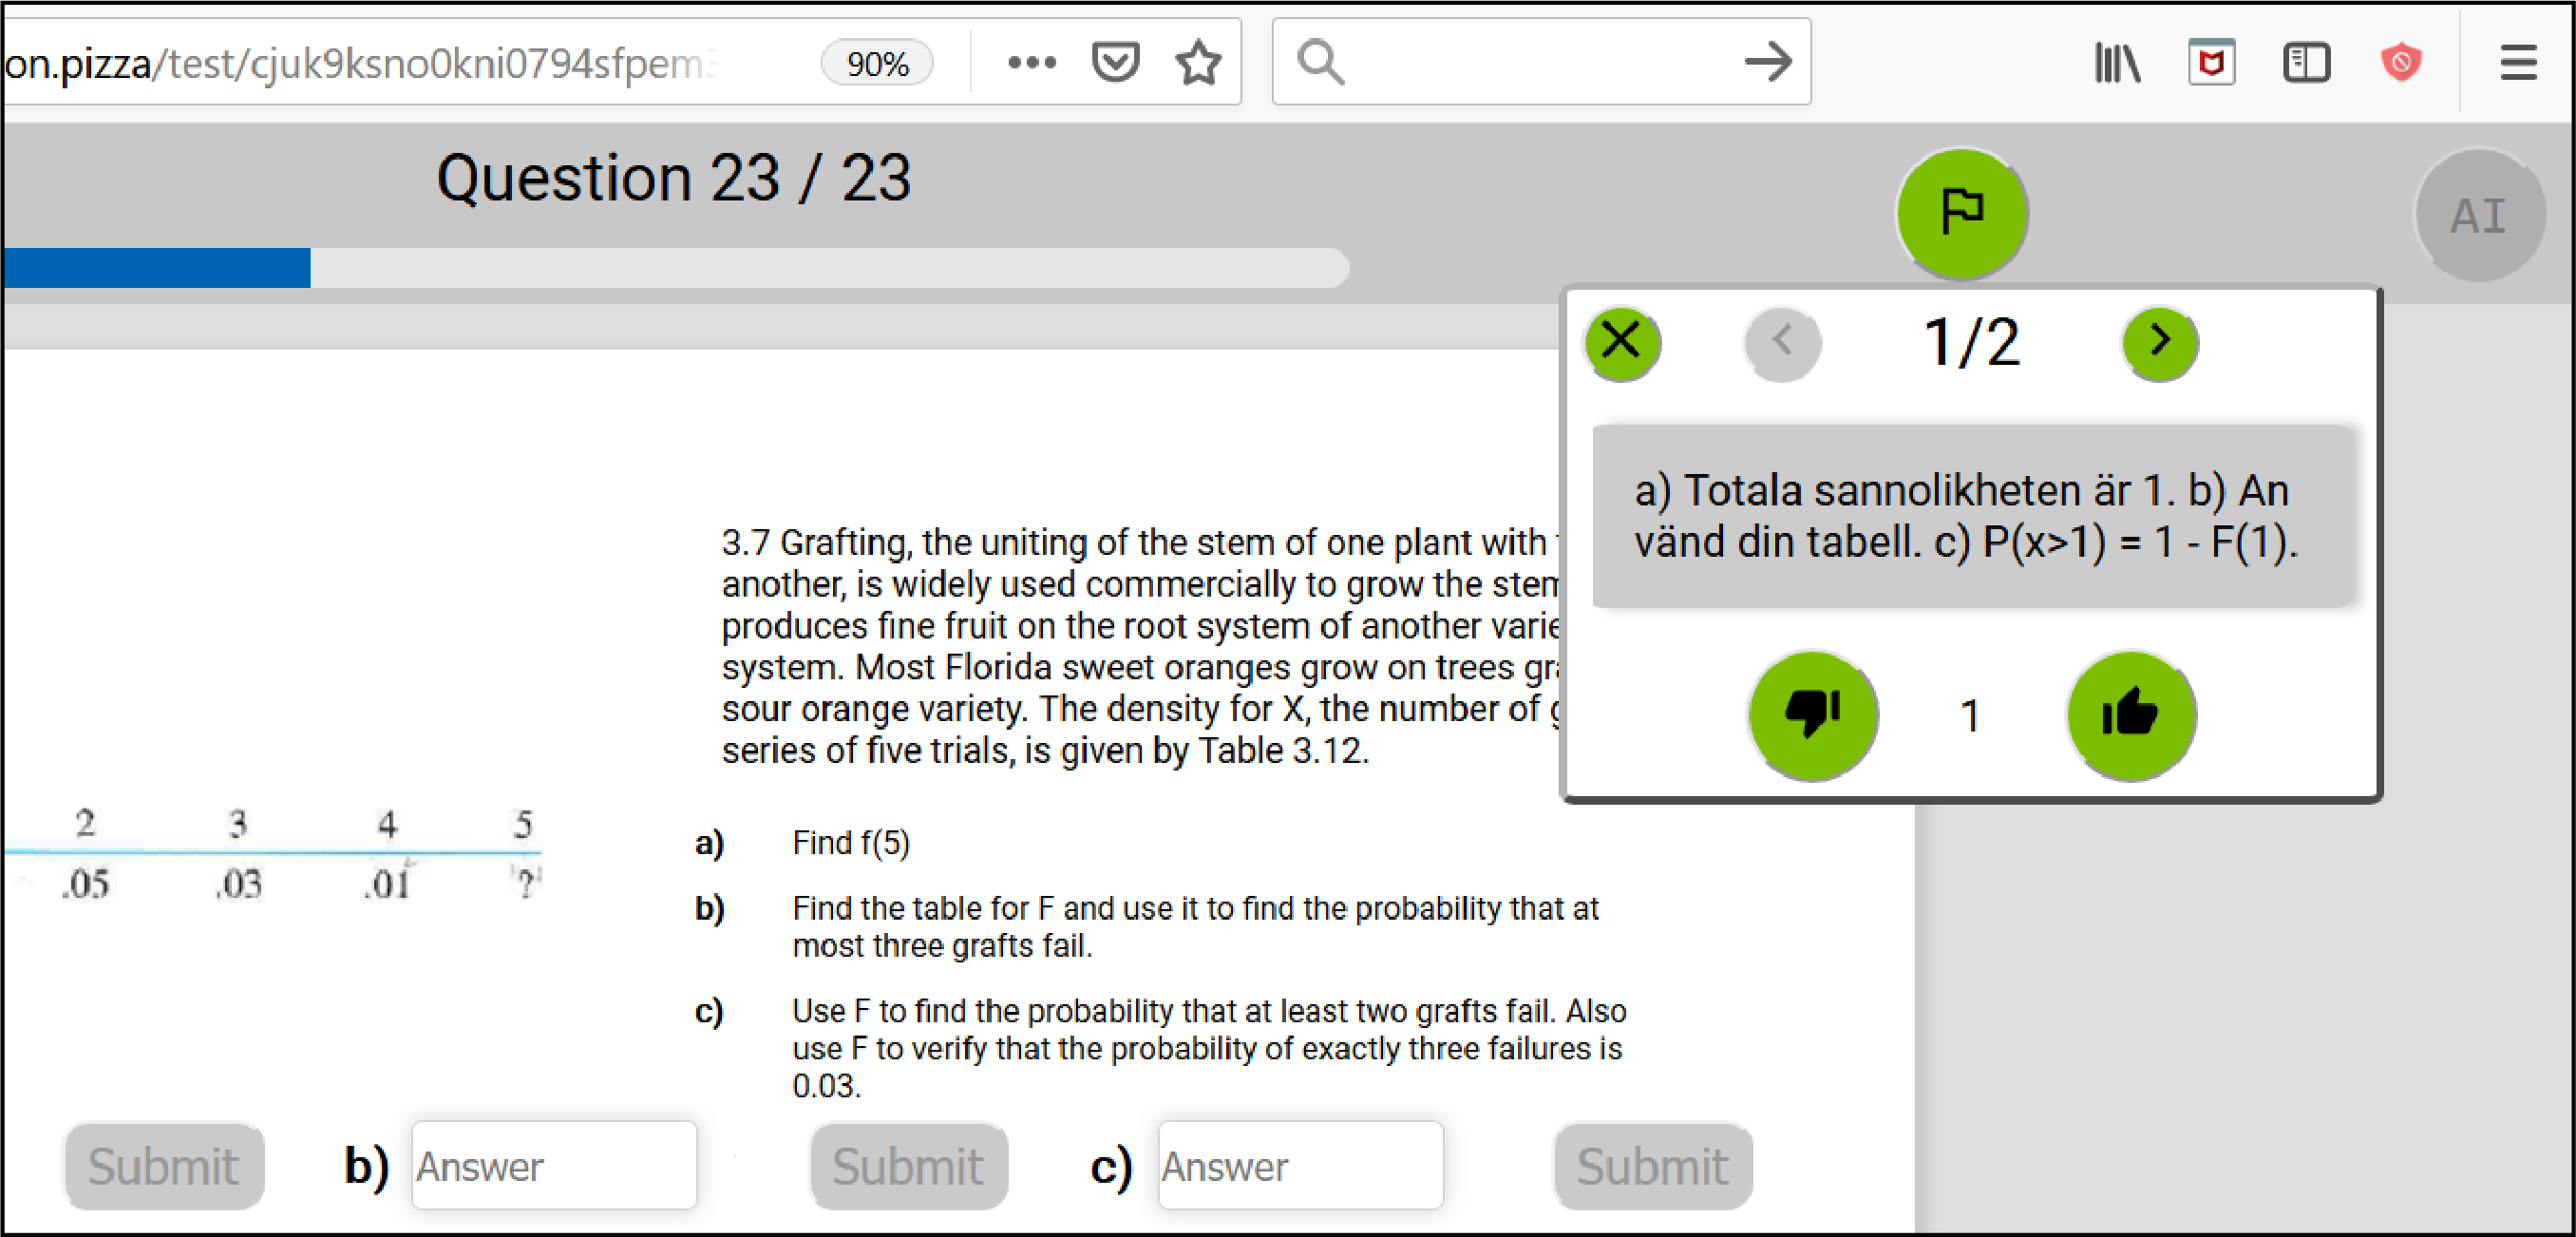
\includegraphics[width=1.0\textwidth]{images/resultpictures/tipsfunktion5.png}
    \caption{Förstorad bild av tipsfunktionen som implementerad i MVP A. Genom att trycka på tipsknappen (flaggan) kan studenten få ett tips om hur uppgiften kan lösas. Notera de två ''tummarna'' som används för att rangordna tipsen.}
    \label{fig:raket6}
\end{figure}


Implementationen av tipsfunktionen förändrade inget av den tidigare beskrivna implementationen för den grundläggande MVP:n, utan motsvarade endast tillagd funktionalitet. Då användaren trycker på tipsknappen hämtas det högst röstade tipset med GraphQL och en dialogruta målas ut där tipsen visas. Användaren kan sedan navigera mellan tipsen, och vid en eventuell navigering hämtas ett nytt tips. Det finns två anledningar till att alla tips inte sparas direkt i cache-minnet. Först och främst hade det inneburit att en användare med enklare erfarenheter av webbutveckling kan komma åt samtliga tips i nätverksloggen, vilket i sin tur innebär att den artificiella intelligensen inte med säkerhet kan veta om användaren tagit hjälp av tipsen. För det andra hade det även försvårat processen att manuellt avgöra hur många tips en användare tagit hjälp av.

För att implementera rangordningen av tips utvecklades ett system där en användare kan rösta på existerande tips. De två ''tummarna'' i figur \ref{fig:raket6} motsvarar då antingen +1 eller -1 i rangordningssystemet. När en användare röstar anropas GraphQL med +1 eller -1. GraphQL användas även då användarna skriver in tips. När en användare besvarat samtliga delfrågor på en uppgift visas en dialogruta där användaren uppmanas att dela sitt mest betydelsefulla tips. Dialogrutan visas i figur \ref{fig:raket7}. Vi har valt att uppmana användaren på ett sådant tydligt sätt för samla in så många tips som möjligt. Ett problem kan annars vara att användaren glömmer att lämna ett tips.

\begin{figure}[hbtp]
    \centering
    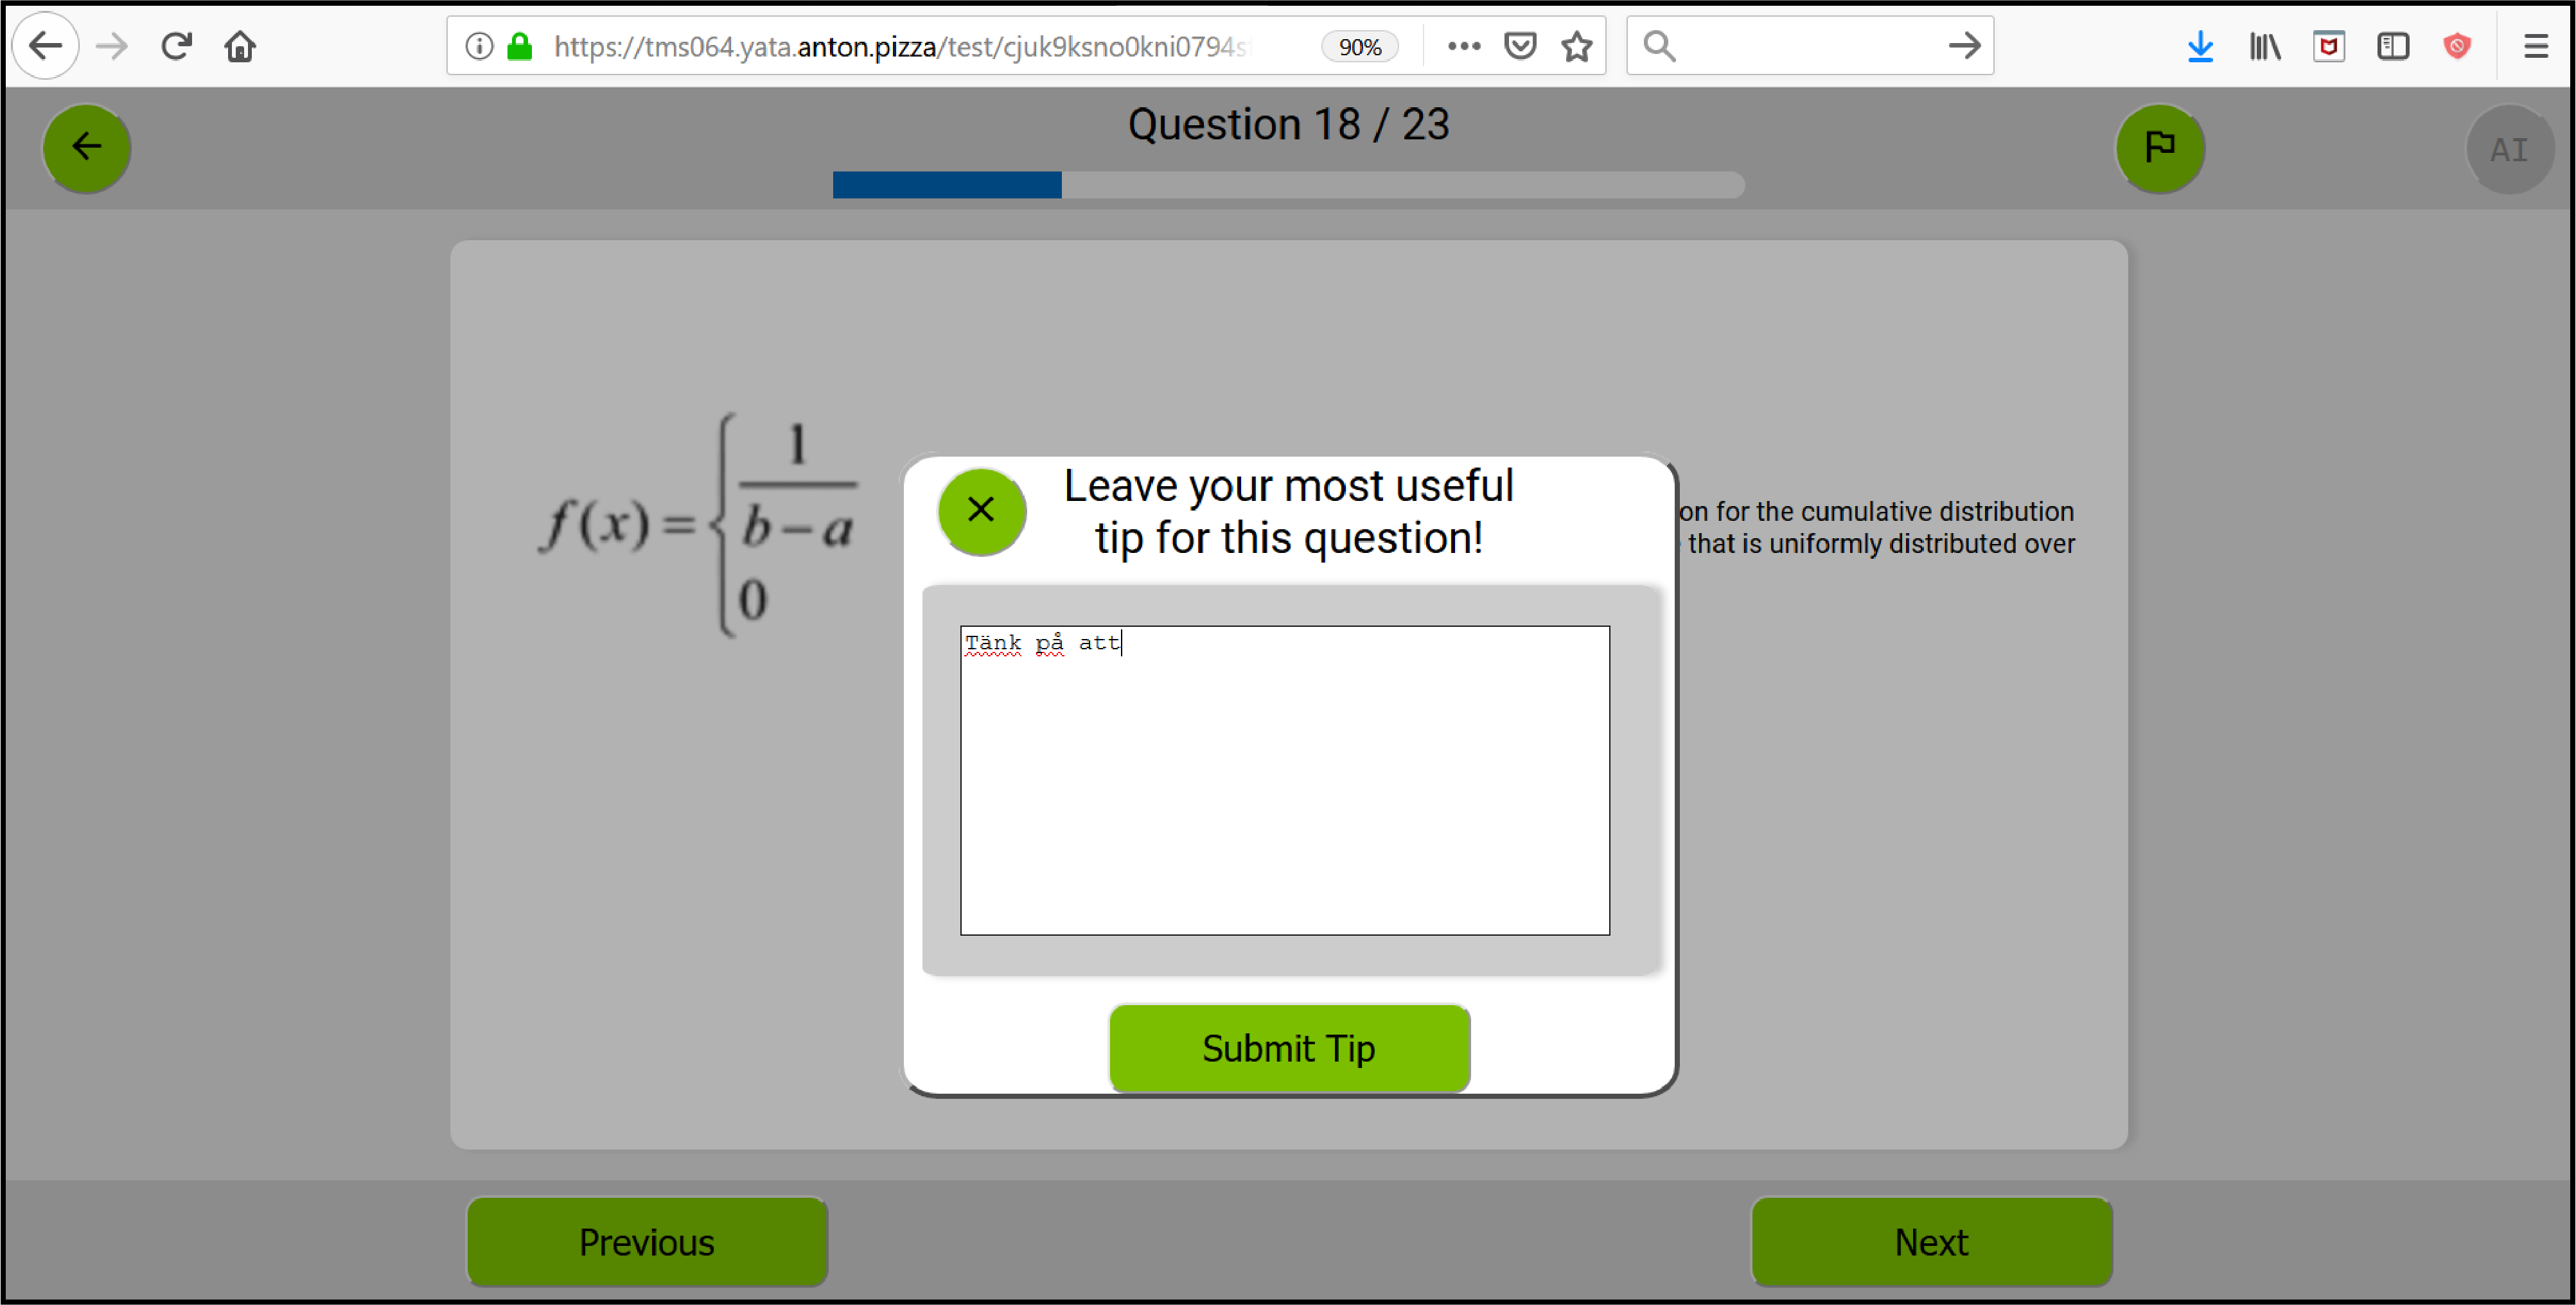
\includegraphics[width=1.0\textwidth]{images/resultpictures/tipsfunktion7.png}
    \caption{När en uppgift är löst får användaren möjlighet att skriva in ett tips för hur uppgiften kan lösas.}
    \label{fig:raket7}
\end{figure}


Vi implementerade och tillgängliggjorde tipsfunktionen i två kurser under läsperiod fyra. Tidigt observerade vi att flera studenter skrivit in tips och gett tips ”tumme upp” vilket indikerar att åtminstone vissa av studenterna finner ett värde i tipsfunktionen. Vad vi också har noterat är att några studenter har skrivit in det korrekta svaret från facit som tips, vilket är ett intressant beteende vars orsak borde undersökas. En rigorös utvärdering av hur tipsfunktionen har fungerat och hur studenterna har använt den har i skrivande stund inte genomförts eftersom kurserna fortfarande pågår.

\section{Ytterligare observationer och diskussion}
\label{sec: webb-D}

Nedan sammanfattar vi gemensamma teman i de två iterationscyklerna, och diskuterar kortfattat funktionalitet och förbättringspunkter. Sist avslutar vi med generella observationer vi gjort kring webbsidans användning i kurserna. 

Ett gemensamt tema i de två iterationscyklerna var att studenterna uppskattade omedelbar återkoppling. Att detta uppskattades framkom i utvärderingen av OpenTA samt i användarstudien av Piazza. Tipsfunktionen är utformad med detta krav i åtanke och erbjuder ögonblicklig hjälp om det finns skrivna tips. Samtidigt är det anonymt att ta hjälp av tipsen eftersom många studenter drog sig för att fråga om hjälp i enlighet med den observerade hierarki. Pedagogiskt kan tipsfunktionen också vara fördelaktig, eftersom studenter kan få hjälp i sin lösningsgång utan att först kolla i facit. Dessutom får studenten som skriver in ett tips möjligheten att reflektera över uppgiften i efterhand, vilket kan vara positivt för inlärningen.

Omedelbar återkoppling identifierades också som ett tydligt krav i utvärderingen av den grundläggande MVP:n. När studenterna interagerar med plattformar som dessa vill de ha direkt och tydlig återkoppling i sin interaktion. I många andra inlärningsprogram som Duolingo och Khan Academy ges positiv återkoppling även vid allra minsta framsteg för att motivera användaren. Därav är ett krav på webbsidan YATA att svarshanteringen är direkt och tydligt återkopplad. I dagsläget har studenterna svårt att skilja på om svaret är inmatat på fel form, om det är syntaxfel, eller om svaret helt enkelt är fel. Detta är något som studenterna vill ha bättre återkoppling på. I vidare utveckling av YATA är ett utvecklingsområde en svarshantering med mer direkt återkoppling.

Ett ytterligare utvecklingsområde är kodstrukturen i implementationen av tipsfunktionen. På grund av arbetets tidsram i iterationscykel 2 prioriterades en kort utvecklingstid. Det kan därför krävas en viss omstrukturering av koden vid vidare utveckling för att bibehålla flexibiliteten. Tipsfunktionen fungerar emellertid tillräckligt bra ur ett användarperspektiv och omstruktureringen hade varit mer omfattande om inte verktyg som React och GraphQL hade använts.

Webbsidan har varit helt frivillig att använda i de kurser där den har varit tillgänglig. Bevisligen har funktionerna i sig varit tillräckliga för att locka studenter till att använda webbsidan. Trots det finns även potential att experimentera med funktionaliteten för att stimulera användningen ytterligare. Exempelvis skulle tipsfunktionen kunna utformas för att ge användaren mer incitament att lämna fler tips genom att användaren får återkoppling när någon röstar upp ett tips den skrivit. YATA visar alltså en potentiellt lovande lösning på problemet att många kör fast i sina lösningsgångar. Vi identifierar därför en mening med att vidareutveckla YATA till en mer stabil och visuellt lockande webbsida genom att iterera de förbättringspunkter vi identifierat i en tredje iterationscykel. 


%%Tipsfunktionen är utformad med tanke på dessa aspekter. Den erbjuder ögonblicklig hjälp om det finns skrivna tips, samtidigt som det är anonymt att ta hjälp av tipsen. Pedagogiskt kan den också vara bättre, eftersom studenter kan få hjälp i sin lösningsgång, utan att först kolla i facit, samt för att den som skriver in ett tips får reflektera över uppgiften i efterhand, vilket kan vara positivt för inlärningen. Vad vi sett från några tidiga observationer av användningen av tipsfunktionen är att studenter har skrivit in tips och gett ”tumme upp” vilket indikerar att åtminstone vissa av studenterna finner ett värde i tipsfunktionen. Vad vi också sett är att vissa skrivit in det korrekta svaret, dvs facit, i tipsrutan, vilket är ett intressant beteende vars orsak borde undersökas. En rigorös utvärdering av hur tipsfunktionen fungerat och hur studenterna använt den bör göras efter läsperiodens slut. 




%%Vad gäller behov och krav för webbplattformar uppskattar, som tidigare nämnt, uppskattar många studenter översikt och struktur. Till exempel, att samla och strukturera upp de rekommenderade uppgifterna på ett ställe samt att det automatiskt hålls koll på vilka uppgifter som  är lösta och inte. Det blir är annars ett extra administrativt moment för studenten. Att webbsidan gör detta innebär att studenterna sparar mer tid, vilket effektiviserar deras studier. När studenterna interagerar med dessa plattformar vill de också ha direkt och tydlig feedback i sin interaktion. I många andra inlärningsprogram till exempel gavs positiv feedback även vid allra minsta framsteg, som en motivationsfaktor för studenten. Ytterligare ett krav på direkt och tydlig feedback har studenterna vad gäller svarshanteringen. I dagsläget har de svårt att skilja på om svaret är inmatat på fel form, om det är syntaxfel, eller om svaret helt enkelt är fel. Detta är något som studenterna vill ha bättre återkoppling på. I vidare utveckling är en svarshantering med mer direkt feedback ett utvecklingsområde. 

%%De behov och krav som identifierats kan i stora drag delas in i två huvudkategorier: behov och krav kring studier i allmänhet samt specifikt kring webbplattformar. Vad vi identifierat kring studier i allmänhet är att studenterna överlag har en vilja att lösa uppgifterna på egen hand. Ibland kör de emellertid fast i lösningsgången och har då ett behov av hjälp på något sätt. Vår tolkning av hierarkin vi identifierade i brukastudien av Piazza är att många värderar svarstiden högre än kvalitén på svaret när de söker efter hjälp. Att maila föreläsaren eller fråga på Piazza hade förmodligen genererat ett svar av hög kvalité, dock är svarstiden ofta långsam. Ett citat från en av intervjuerna är ''det känns bättre att googla i fem minuter än att vänta i fem minuter'', vilket visar på ett tydligt behov av att få hjälpen direkt. Ytterligare något vi observerade var att studenterna överlag drar sig för att ställa frågor i större öppna forum, men om de gör det är anonymitet ett krav. Det finns en viss rädsla för att fråga om hjälp i mer offentliga sammanhang, även om det är i en digital miljö som ett forum. Studenterna känner sig mer trygga att fråga om hjälp i en mindre gruppchatt med sina nära vänner till exempel. Allra först dock, söker många hjälp via Google. Förmodligen för att det är mest lättillgängligt, men kanske också för att det inte är en social miljö på samma sätt som ett forum eller en gruppchatt. 

